% ══════════════════════════════════════════════════════════════════════════════
% CHAPTER 5: RESULTS & ANALYSIS (draft)
% ══════════════════════════════════════════════════════════════════════════════

\section*{CHAPTER 5: RESULTS}
\addcontentsline{toc}{section}{\numberline{}CHAPTER 5: RESULTS}
\setcounter{section}{5}
\setcounter{subsection}{0}
\setcounter{figure}{0}
\setcounter{table}{0}

\subsection{Feature engineering and classical models}

\subsubsection{Impact of Text Preprocessing}

Section 2.3 shows that issue bodies are roughly 40\% non-prose, and that the noise is class-correlated. We cross-validated the same logistic regression pipeline across all eighteen combinations of cleaning level, title weight and truncation (Table~\ref{tab:cleaning_ablation})

\begin{table}[H]
\centering
\caption{Cross-validated performance comparison across preprocessing cleaning levels.}
\label{tab:cleaning_ablation}
\vspace{0.5em}
\begin{tabular}{l c c}
\hline
Cleaning level & mean macro F1 & best macro F1 \\
\hline
\texttt{raw} & 0.7446 & 0.7472 \\
\texttt{light} & 0.7434 & 0.7472 \\
\textbf{\texttt{full}} & \textbf{0.7326} & \textbf{0.7364} \\
\hline
\end{tabular}
\end{table}

Cleaning level \textbf{\texttt{full} is the worst of the three}, costing roughly 0.011 on the mean and 0.011 on the best configuration -- consistent across every title weight and truncation setting tested, without a single exception.

The reason is in what \texttt{full} removes. Stop-word removal deletes \textit{would}, \textit{could}, \textit{should}, \textit{please} and \textit{nice}; lemmatisation collapses tense. Those are precisely the modal and evaluative words that Section 2.4 identified as the signature of a feature request. The cleaning was removing the signal along with the noise.

\subsubsection{Hyperparameter Optimization}

Cross-validated grid search over regularization strength, n-gram range and minimum document frequency, on the training split only (Table~\ref{tab:hyperparameter_tuning})

\begin{table}[H]
\centering
\caption{Best hyperparameter configurations and cross-validation scores for linear models.}
\label{tab:hyperparameter_tuning}
\vspace{0.5em}
\begin{tabular}{l l c}
\hline
Model & best configuration & CV macro F1 \\
\hline
Logistic regression & \texttt{C=10}, bigrams, \texttt{min\_df=2} & 0.7481 \\
Linear SVM & \texttt{C=1}, bigrams, \texttt{min\_df=1} & 0.7484 \\
\hline
\end{tabular}
\end{table}

\textbf{Tuning gained almost nothing.} The best and fifth-best configurations differ by about 0.002 against a fold-to-fold standard deviation of roughly 0.029. Only the bi-gram setting clearly exceeds the noise.

One process note belongs here. The grid was first run under \texttt{full} cleaning, and the winning \texttt{min\_df} changed once the ablation moved the pipeline to \texttt{light}. Hyperparameters and preprocessing are not independent, and re-tuning after altering the pipeline is not optional.

\subsubsection{Classical results}

From Table~\ref{tab:classical_models_results}, the three linear models cluster within 0.007 of each other; naive Bayes trails by 0.045. Random forest is the only model whose test score falls materially below its cross-validation score, which is expected -- trees cope poorly with the very high-dimensional sparse features TF-IDF produces, and the result is a finding rather than a bug.

\begin{table}[H]
\centering
\caption{Evaluation results of classical machine learning models on TF-IDF features.}
\label{tab:classical_models_results}
\vspace{0.5em}
\begin{tabular}{l c c c}
\hline
Model & CV macro F1 & test F1 & AUC \\
\hline
\textbf{TF-IDF + Logistic Regression (tuned)} & 0.7446 $\pm$ 0.0398 & \textbf{0.7603} & 0.9018 \\
TF-IDF + Linear SVM & 0.7426 $\pm$ 0.0367 & 0.7583 & --- \\
TF-IDF + Logistic Regression & 0.7478 $\pm$ 0.0409 & 0.7576 & 0.9016 \\
TF-IDF + Linear SVM (tuned) & 0.7499 $\pm$ 0.0430 & 0.7531 & --- \\
TF-IDF + Naive Bayes & 0.6919 $\pm$ 0.0334 & 0.7140 & 0.8713 \\
TF-IDF + Complement NB & 0.6902 $\pm$ 0.0311 & 0.7012 & 0.8673 \\
TF-IDF + Random Forest & 0.7252 $\pm$ 0.0316 & 0.6978 & 0.8630 \\
\hline
\end{tabular}
\end{table}

Note the fold-to-fold standard deviations, all around 0.03--0.04. \textbf{Every difference within the top four rows is inside one standard deviation.} The ordering among them should not be over-interpreted.

\subsection{Validation curves and overfitting control}

With 300 training issues per project, overfitting appears quickly.

\begin{table}[H]
\centering
\caption{Training metrics, early stopping status, and loss progressions for neural models.}
\label{tab:neural_training_progression}
\vspace{0.5em}
\begin{tabular}{l c c c c p{4.2cm}}
\hline
Model & Epochs & Best & Stopped? & Train Loss & Validation Loss \\
\hline
FFNN (TF-IDF) & 23 & 15 & yes & $1.099 \rightarrow 0.007$ & $1.093 \rightarrow 0.579$ (min 0.572) \\
CNN (embeddings) & 38 & 30 & yes & $1.267 \rightarrow 0.053$ & $0.989 \rightarrow 0.574$ (min 0.513) \\
\hline
\end{tabular}
\end{table}

% \textit{(Figures: \texttt{learning\_curve\_ffnn\_tf\_idf.png}, \texttt{learning\_curve\_cnn\_embeddings.png})}

\begin{figure}[htbp]
    \centering
    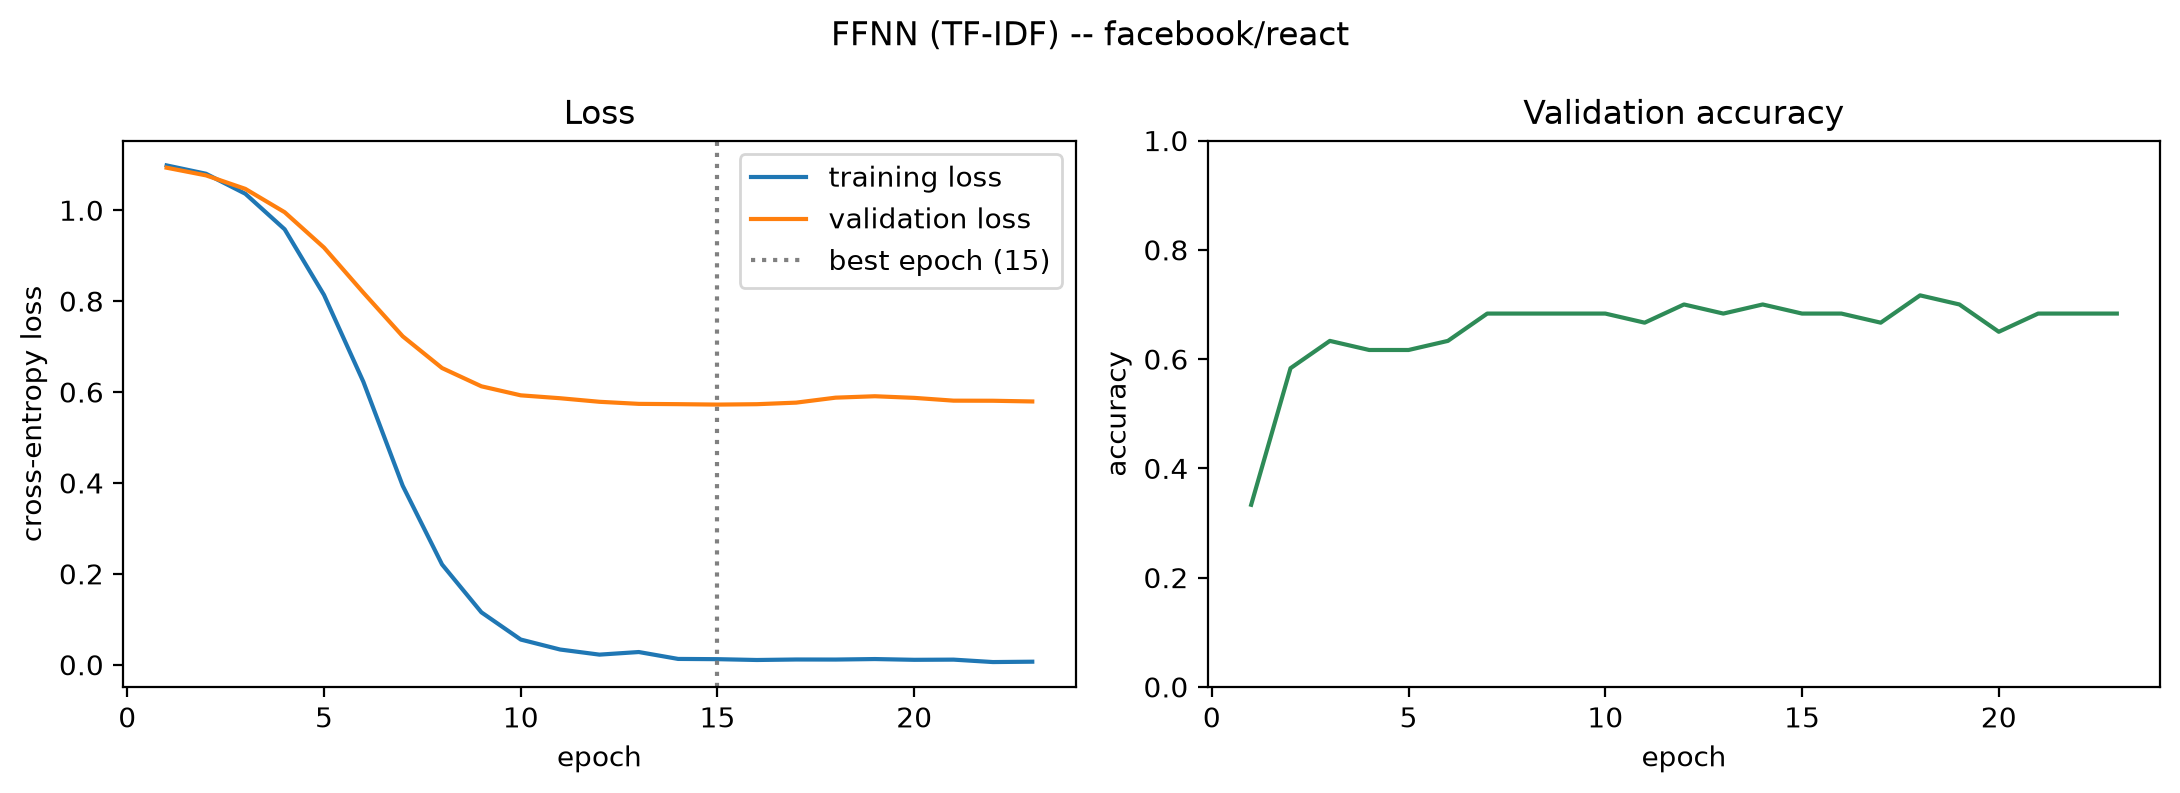
\includegraphics[width=0.95\textwidth]{results/figures/learning_curve_ffnn_tf_idf.png}
    \caption{FFNN (TF-IDF) learning curve.}
    \label{fig:curve_ffnn}
    
    \vspace{0.5em}
    
    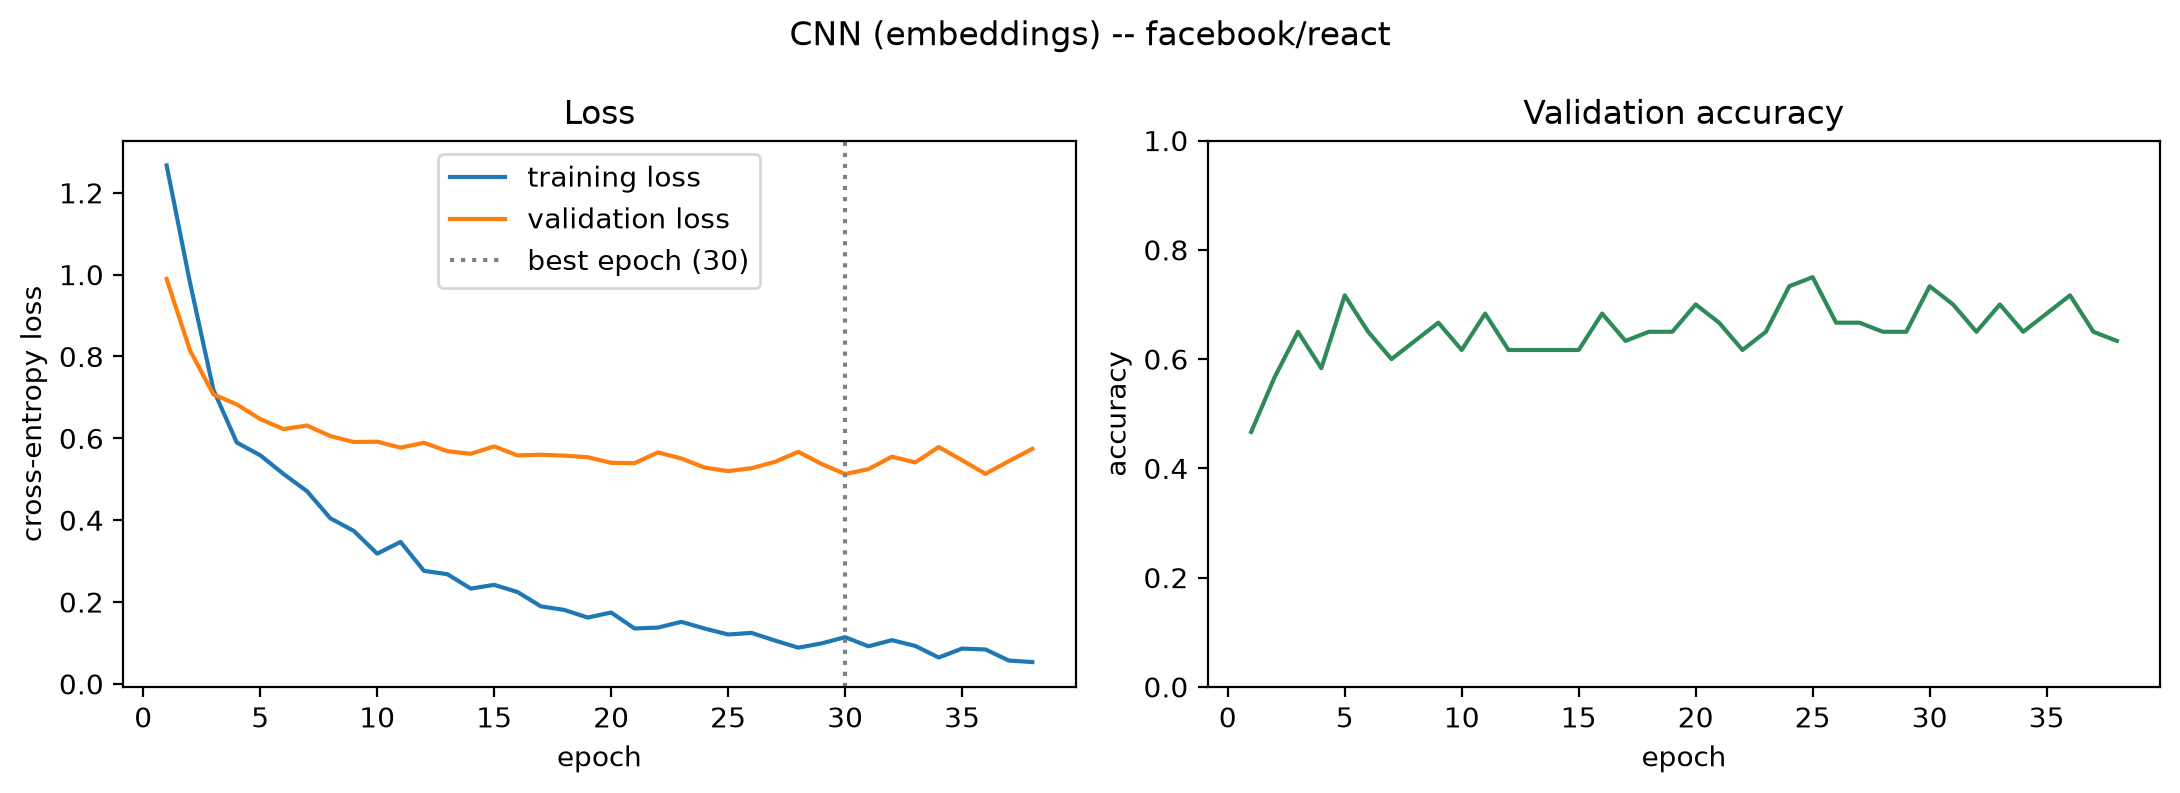
\includegraphics[width=0.95\textwidth]{results/figures/learning_curve_cnn_embeddings.png}
    \caption{CNN (embeddings) learning curve.}
    \label{fig:curve_cnn}
\end{figure}

The FFNN drives training loss essentially to zero -- 0.007 -- while validation loss bottoms out at 0.572 and then rises. That is the textbook example of a model that has stopped generalising and started memorising, and it happens within fifteen epochs on 240 training examples.

The CNN overfits more slowly, reaching its best epoch at 30. It has fewer effective parameters acting on each input position and must learn its embedding table from scratch, so it takes longer to reach the point of memorisation -- and reaches a lower validation minimum (0.513) when it does.

Both use early stopping with a patience of 8 epochs and restore the weights from the best epoch rather than the last. This is the primary overfitting remedy in our neural pipeline; the second is the architecture size, which the dataset forces to be small; the third is the cross-validation framework of Section 4.3.

\begin{table}[H]
\centering
\caption{Test set performance metrics for neural network architectures.}
\label{tab:neural_test_results}
\vspace{0.5em}
\begin{tabular}{l c c}
\hline
Model & test F1 & AUC \\
\hline
CNN (embeddings) & 0.7438 & 0.8885 \\
FFNN (TF-IDF) & 0.7424 & 0.8926 \\
\hline
\end{tabular}
\end{table}

\textbf{Neither neural model beats TF-IDF with logistic regression (0.7603).} The FFNN consumes exactly the same features as the classical pipelines and scores 0.018 lower; the CNN, which learns its own representation, scores 0.017 lower. With 300 training issues per project there is not enough data to learn a better representation than TF-IDF already provides.

\subsection{Per-project versus global training}

The competition requires five classifiers, each trained on 300 issues, rather than one trained on 1,500. Section 2.5 predicted this would help, on the grounds that cross-project vocabulary overlap is low (Jaccard 0.266). We tested it directly, training each model both ways and scoring both per project, the results are being shown in Table~\ref{tab:per_project_vs_global}

% \begin{table}[h]
% \centering
% \begin{tabular}{l c c c c}
% \hline
% Model & per-project & global & difference & projects where per-project wins \\
% \hline
% Naive Bayes (from scratch, \texttt{full}) & 0.6679 & 0.6003 & \textbf{+0.0676} & 5 / 5 \\
% Naive Bayes (from scratch, \texttt{light}) & 0.7046 & 0.6401 & +0.0645 & 4 / 5 \\
% TF-IDF + Naive Bayes & 0.7140 & 0.6822 & +0.0318 & 4 / 5 \\
% TF-IDF + Logistic Regression (tuned) & 0.7603 & 0.7621 & $-$0.0019 & 2 / 5 \\
% TF-IDF + Linear SVM (tuned) & 0.7531 & 0.7639 & \textbf{$-$0.0108} & 2 / 5 \\
% \hline
% \end{tabular}
% \end{table}

\begin{table}[H]
\centering
\caption{Performance comparison between per-project and globally trained models.}
\label{tab:per_project_vs_global}
\vspace{0.5em}
\begin{tabular}{l c c c c}
\hline
Model & Per-project & Global & Difference & \begin{tabular}{@{}c@{}}Per-project \\ wins\end{tabular} \\
\hline
Naive Bayes (from scratch, \texttt{full})  & 0.6679 & 0.6003 & \textbf{+0.0676} & 5 / 5 \\
Naive Bayes (from scratch, \texttt{light}) & 0.7046 & 0.6401 & +0.0645          & 4 / 5 \\
TF-IDF + Naive Bayes                      & 0.7140 & 0.6822 & +0.0318          & 4 / 5 \\
TF-IDF + Logistic Regression (tuned)      & 0.7603 & 0.7621 & $-$0.0019        & 2 / 5 \\
TF-IDF + Linear SVM (tuned)               & 0.7531 & 0.7639 & \textbf{$-$0.0108}& 2 / 5 \\
\hline
\end{tabular}
\end{table}

\textbf{The prediction holds for weak models and fails for strong ones.} The per-project advantage is large for naive Bayes (+0.068), halves for TF-IDF naive Bayes (+0.032), and reverses entirely for the regularised linear models, which do slightly \textit{better} trained globally on five times the data.

The mechanism is regularisation and feature weighting. Naive Bayes has neither: every term contributes to the posterior in proportion to its frequency, so the project-specific technical vocabulary documented in Section 2.4 -- \texttt{cudatoolkit}, \texttt{liveserver}, \texttt{geforce} -- actively misleads a globally trained model, because those terms correlate with a class \textit{within one project} and carry no such signal across projects. A regularised linear model on TF-IDF can down-weight exactly those terms, at which point the fivefold increase in training data becomes worth more than the specialisation.

\subsection{Decomposing the published baseline}

\subsubsection{The reproduction}

Our implementation of the published method reaches \textbf{0.8108} against the published \textbf{0.8270}, short by 0.0162.

\subsubsection{Where the performance comes from}

The frozen-encoder configuration -- pretrained encoder, logistic-regression head, no fine-tuning -- is precisely SetFit with the contrastive step removed. Running both encoders in both configurations decomposes the baseline, which being shown in Tabel~\ref{tab:baseline_decomposition}

\begin{table}[H]
\centering
\caption{Factorial decomposition of encoder capacity versus contrastive fine-tuning effect.}
\label{tab:baseline_decomposition}
\vspace{0.5em}
\begin{tabular}{l c c c}
\hline
Configuration & MiniLM & MPNet & encoder effect \\
\hline
Frozen encoder + LogReg & 0.7057 & 0.7557 & \textbf{+0.0500} \\
SetFit @ \texttt{batch=8, seq=128} & 0.7816 & 0.8108 & \textbf{+0.0292} \\
\textbf{fine-tuning effect} & \textbf{+0.0759} & \textbf{+0.0551} & \\
\hline
\end{tabular}
\end{table}

\textbf{Contrastive fine-tuning is worth +0.0759 on a fixed encoder} -- with everything else held constant. It is the largest single lever identified in this project, and roughly two and a half times the effect of doubling the encoder's depth and width.

% \subsubsection{A prediction that failed, and a correction that was itself wrong}

% This measurement went through three stages, and we report all three because the process is the substantive contribution.

% \textbf{Stage 1 -- projection.} From the frozen models and the first fine-tuned run, we measured an encoder effect of +0.0500 and a fine-tuning effect of +0.0925, and projected SetFit-on-MPNet at \textbf{0.8482} -- above the published baseline.

% \textbf{Stage 2 -- measurement.} The actual value was \textbf{0.8102}. The projection was wrong by 0.038, and wrong about the conclusion. Taken at face value the encoder appeared worth only +0.0120 after fine-tuning against +0.0500 frozen, implying severe sub-additivity.

% \textbf{Stage 3 -- the confound.} That comparison was not controlled. MiniLM had run at \texttt{batch\_size=16} with the encoder's own \texttt{max\_seq\_length} of 256; MPNet required 8 and 128 to fit in 12 GB of GPU memory, so the handicap fell on MPNet. Re-running MiniLM at MPNet's exact settings gives \textbf{0.7816} -- meaning \textbf{the reduced training settings cost 0.0166 on their own}, and the true encoder effect is +0.0286, not +0.0120.

% Sub-additivity is real but far milder than stage 2 suggested: the encoder retains \textbf{57\%} of its frozen value after fine-tuning, not 24\%.

% Two methodological points follow, in order of importance:

% \begin{enumerate}
%     \item \textbf{Effects measured separately were assumed to compose, and they did not.} Task adaptation and model capacity are partly substitutes -- adapting a small encoder recovers most of what a larger general-purpose one provides.
%     \item \textbf{The first correction was itself overstated, because the comparison behind it was confounded.} Only the matched re-run settled it.
% \end{enumerate}

% A practical corollary: \textbf{training settings matter about as much as encoder size here} -- 0.0166 for batch and sequence length against 0.0286 for doubling the encoder. A result reported without its batch size and sequence length is not comparable with another.

\subsection{Ensembles}

Sections 5.1 and 5.4 produce models of similar strength by different means, which invites checking whether they fail in the same places. It can be clearly seen that they do not in Table~\ref{tab:model_complementarity}

\begin{table}[H]
\centering
\caption{Per-repository F1 score comparison highlighting lexical and semantic model complementarity.}
\label{tab:model_complementarity}
\vspace{0.5em}
\begin{tabular}{l c c c c c c}
\hline
 & react & tensorflow & vscode & bitcoin & opencv & spread \\
\hline
TF-IDF + LogReg (tuned) & \textbf{0.8334} & \textbf{0.8155} & 0.7234 & 0.6793 & 0.7496 & 0.154 \\
Frozen MPNet + LogReg & 0.8017 & 0.7228 & \textbf{0.7566} & \textbf{0.7279} & \textbf{0.7696} & \textbf{0.079} \\
\hline
\end{tabular}
\end{table}

TF-IDF wins the two easiest projects, MPNet all three hardest, and MPNet's spread across projects is half as wide. Lexical overlap between training and test issues is high within an easy project and low within a hard one, which is where a pretrained semantic representation works. Two models of equal average strength failing in different places is the precondition for an ensemble.

\begin{table}[H]
\centering
\caption{Overall test set performance of soft-voting ensemble combinations.}
\label{tab:ensemble_results}
\vspace{0.5em}
\begin{tabular}{l c c c}
\hline
Ensemble & test F1 & AUC & gain over best member \\
\hline
\textbf{SetFit + TF-IDF + MPNet} & \textbf{0.8168} & \textbf{0.9319} & +0.0066 \\
SetFit + TF-IDF & 0.8053 & 0.9244 & +0.0071 \\
TF-IDF + MPNet + CNN & 0.7909 & 0.9245 & +0.0306 \\
TF-IDF + MPNet & 0.7838 & 0.9198 & +0.0235 \\
\hline
\end{tabular}
\end{table}

Every ensemble beats its best member. The GPU-free combination of TF-IDF, frozen MPNet and the CNN reaches 0.7909 -- within 0.007 of a full SetFit reproduction, at no fine-tuning cost.

The best ensemble reaches \textbf{0.8168} and attains the \textbf{highest AUC of any model measured, 0.9319}, above even SetFit-on-MPNet's 0.9195. Its ranking of the classes is better than its argmax decision suggests, which mean a tuned decision threshold might recover further.

\subsection{Final results}
Table~\ref{tab:final_leaderboard} contextualizes all evaluated configurations against the official competition benchmark.
\begin{table}[H]
\centering
\caption{Final overall benchmark leaderboard across all evaluated models on the test split.}
\label{tab:final_leaderboard}
\vspace{0.5em}
\begin{tabular}{l c c c}
\hline
Model & overall F1 & AUC & vs baseline \\
\hline
\textbf{SetFit (NLBSE'24 published baseline)} & \textbf{0.8270} & --- & --- \\
\textbf{Ensemble (SetFit + TF-IDF + MPNet)} & \textbf{0.8168} & \textbf{0.9319} & $-$0.0102 \\
SetFit (MPNet) & 0.8108 & 0.9195 & $-$0.0162 \\
Ensemble (SetFit + TF-IDF) & 0.8053 & 0.9244 & $-$0.0217 \\
SetFit (reproduction, MiniLM) & 0.7982 & 0.9181 & $-$0.0288 \\
Ensemble (TF-IDF + MPNet + CNN) & 0.7909 & 0.9245 & $-$0.0361 \\
Ensemble (TF-IDF + MPNet) & 0.7838 & 0.9198 & $-$0.0432 \\
SetFit (MiniLM, matched settings) & 0.7816 & 0.9144 & $-$0.0454 \\
TF-IDF + Logistic Regression (tuned) & 0.7603 & 0.9018 & $-$0.0667 \\
TF-IDF + Linear SVM & 0.7583 & -- & $-$0.0687 \\
TF-IDF + Logistic Regression & 0.7576 & 0.9016 & $-$0.0694 \\
Frozen MPNet + LogReg & 0.7557 & 0.8970 & $-$0.0713 \\
TF-IDF + Linear SVM (tuned) & 0.7531 & -- & $-$0.0739 \\
CNN (embeddings) & 0.7438 & 0.8885 & $-$0.0832 \\
FFNN (TF-IDF) & 0.7424 & 0.8909 & $-$0.0846 \\
TF-IDF + Naive Bayes & 0.7140 & 0.8713 & $-$0.1130 \\
Frozen MiniLM + LogReg & 0.7057 & 0.8837 & $-$0.1213 \\
TF-IDF + Complement NB & 0.7012 & 0.8673 & $-$0.1258 \\
TF-IDF + Random Forest & 0.6978 & 0.8630 & $-$0.1292 \\
Naive Bayes (from scratch) & 0.6679 & 0.8246 & $-$0.1591 \\
Keyword rules & 0.5395 & --- & $-$0.2875 \\
Random (stratified) & 0.3348 & --- & $-$0.4922 \\
Majority class & 0.1667 & --- & $-$0.6603 \\
\hline
\end{tabular}
\end{table}

% \textit{(Full per-repository table: \texttt{final\_leaderboard.tex})}

\textbf{Our best result closes 98.5\% of the distance from a majority-class classifier to the published baseline.} We do not beat it overall; the remaining 0.0102 is real, and Section 7 discusses what would likely close it.

Three observations across the table:

\textbf{Every purely lexical model lands between 0.70 and 0.76} regardless of classifier family -- naive Bayes, SVM, logistic regression, random forest, a feed-forward network and a CNN. The things that moved the number were a better representation (+0.050 for a larger encoder) and adapting it to the task (+0.076 for fine-tuning), not the choice of classifier.

\textbf{AUC and F1 do not rank models identically.} The best ensemble has the highest AUC (0.9319) but only the second-highest F1. Reporting both, as the course requires, surfaces information that either alone would hide.

\textbf{\texttt{bitcoin/bitcoin} is hardest for almost every model}, and for the published baseline too (0.7555, its lowest per-project score). Project difficulty is a property of the data rather than of any approach -- which matters before attributing a low per-project score to a model.